\subsection{Restaurant use cases}
\todo[inline]{check if covered reqs are actually covered by use cases}
\todo[inline]{check if order of left column is the same in all use cases}

\noindent \textbf{x. Use case: Create a new menu}
\todo[inline]{add names of use cases to extension point}
\begin{center}
  \begin{tabular}{| l | p{10.75cm} | }
    \hline
    Actor         & Restaurant \\
    \hline
    Description   & A restaurant employee wants to create a new menu. \\
    \hline
    Covers        & R2.8, R2.9, R2.12, R2.14  \\
    \hline
    Precondition  & A restaurant employee is logged in to the application. \\
    \hline
    Postcondition & A new menu is created and saved. \\
    \hline
    Scenario      &
    \begin{minipage}[t]{\linewidth}
      \begin{enumerate}[leftmargin=*,nosep,before=\vspace{-0.575\baselineskip},after=\strut]
        \item The application displays a screen with an empty menu. \textbf{A1}
        \item The restaurant employee specifies the name of the menu.
        \item The restaurant employee specifies when will the menu be valid. \textbf{Extension point - UCx}
        \item The restaurant employee specifies categories of the menu. \textbf{A2}
        \item The restaurant employee adds food items to the categories of the menu.
        \item The restaurant employee presses the button for saving the menu.
        \item The application saves the menu.
      \end{enumerate}
    \end{minipage}
    \\
    \hline
    Alternatives &
    \begin{minipage}[t]{\linewidth}
      \begin{description}[nosep,after=\strut]
        \item [A1:] The restaurant employee chooses to use an existing menu as the starting point for creating the new menu. The application inserts contents of the existing menu to the menu which is being created.
        \item [A2:] The restaurant employee does not add any categories to the menu. The application creates a menu without categories.
      \end{description}
    \end{minipage}
    \\
    \hline
  \end{tabular}
  \newline
\end{center}

\newpage

\noindent \textbf{x. Use case: Add a food item to a menu} 
\todo[inline]{add use case number in extension point}
\begin{center}
  \begin{tabular}{| l | p{10.75cm} | }
    \hline
    Actor         & Restaurant \\
    \hline
    Description   & A restaurant employee is creating a menu and wants to add a food item to it. \\
    \hline
    Covers        & R2.10, R2.13, R2.15, R2.16 \\
    \hline
    Precondition  & The restaurant employee is logged in to the application and has started the process of creation of a new menu. \\
    \hline
    Postcondition & A food item is added to a menu which is beaing created. \\
    \hline
    Scenario      &
    \begin{minipage}[t]{\linewidth}
      \begin{enumerate}[leftmargin=*,nosep,before=\vspace{-0.575\baselineskip},after=\strut]
        \item The restaurant employee specifies the name, price, weight or volume and description of the menu item. 
        \item The restaurant employee specifies the menu item's ingredients.
        \item The application adds allergens to the menu item. \textbf{Extension point - UCx}
        \item The restaurant employee presses the button for adding the item to the menu. 
        \item The application adds the item to the menu. \textbf{A1}
      \end{enumerate}
    \end{minipage}
    \\
    \hline
    Alternatives  &
    \begin{minipage}[t]{\linewidth}
      \begin{description}[nosep,after=\strut]
        \item [A1:] The restaurant employee did not specify the name of the menu item. The application prompts the restaurant employee to add this information. The application does not add the item to the menu until the name of the item is specified.
      \end{description}
    \end{minipage}
    \\
    \hline
  \end{tabular}
  \newline
\end{center}

\noindent \textbf{x. Use case: Warn my guests about allergens in the foods I serve}
\todo[inline]{add use case number in extends column}
\begin{center}
  \begin{tabular}{| l | p{10.75cm} | }
    \hline
    Actor         & Restaurant \\
    \hline
    Description   & A restaurant employee wants to have accurate allergen information in a menu. \\
    \hline
    Covers        & R2.11, R2.12 \\
    \hline
    Extends       & Add a food item to the menu  \\
    \hline
    Precondition  & The restaurant employee has added ingredients to a menu item. \\
    \hline
    Postcondition & A menu item contains information about its allergens. \\
    \hline
    Scenario      &
    \begin{minipage}[t]{\linewidth}
      \begin{enumerate}[leftmargin=*,nosep,before=\vspace{-0.575\baselineskip},after=\strut]
        \item The application inserts allergens to the menu item based on its ingredients.
      \end{enumerate}
    \end{minipage}
    \\
    \hline
  \end{tabular}
  \newline
\end{center}

\noindent \textbf{x. Use case: Create a stable menu}
\todo[inline]{add use case number in extends column}
\begin{center}
  \begin{tabular}{| l | p{10.75cm} | }
    \hline
    Actor        & Restaurant \\
    \hline
    Description  & A restaurant employee wants to set that a menu will be valid every day of the week. \\
    \hline
    Covers & R2.2 \\
    \hline
    Extends       &  x: Create a new menu \\
    \hline
    Precondition  & The restaurant employee is logged in to the application and has started the process of creation of a new menu. \\
    \hline
    Postcondition & The menu's date of validity is configured so that it is valid every day of the week. \\
    \hline
    Scenario     &
    \begin{minipage}[t]{\linewidth}
      \begin{enumerate}[leftmargin=*,nosep,before=\vspace{-0.575\baselineskip},after=\strut]
        \item The restaurant employee checks the option that the menu is a stable menu.
        \item The application sets that the menu will be valid for every day of the week.
      \end{enumerate}
    \end{minipage}
    \\
    \hline
  \end{tabular}
  \newline
\end{center}

\noindent \textbf{x. Use case: Create a list of beverages}
\todo[inline]{add use case number in extends column}
\begin{center}
  \begin{tabular}{| l | p{10.75cm} | }
    \hline
    Actor        & Restaurant \\
    \hline
    Description  & A restaurant employee wants to set that a list of beverages will be valid every day of the week. \\
    \hline
    Covers & R2.3 \\
    \hline
    Extends       &  x: Create a new menu \\
    \hline
    Precondition  & The restaurant employee is logged in to the application and has started the process of creation of a new menu. \\
    \hline
    Postcondition & The list of beverages' date of validity is configured so that it is valid every day of the week. \\
    \hline
    Scenario     &
    \begin{minipage}[t]{\linewidth}
      \begin{enumerate}[leftmargin=*,nosep,before=\vspace{-0.575\baselineskip},after=\strut]
        \item The restaurant employee checks the option that the menu is a list of beverages.
        \item The application sets that the list of beverages will be valid for every day of the week.
      \end{enumerate}
    \end{minipage}
    \\
    \hline
  \end{tabular}
  \newline
\end{center}

\noindent \textbf{x. Use case: Create a daily menu for tomorrow}
\todo[inline]{add use case number in extends column}
\begin{center}
  \begin{tabular}{| l | p{10.75cm} | }
    \hline
    Actor        & Restaurant \\
    \hline
    Covers        & R2.1 \\
    \hline
    Extends       &  x: Create a new menu \\
    \hline
    Precondition  & The restaurant employee is logged in to the application and has started the process of creation of a new menu. \\
    \hline
    Postcondition & The menu's date and time of validity is configured so that it will be valid for a certain day and hour span. \\
    \hline
    Scenario     &
    \begin{minipage}[t]{\linewidth}
      \begin{enumerate}[leftmargin=*,nosep,before=\vspace{-0.575\baselineskip},after=\strut]
        \item The restaurant employee selects the day for which the menu will be valid.
        \item The restaurant employee specifies the time range for which the menu will be served that day.
      \end{enumerate}
    \end{minipage}
    \\
    \hline
  \end{tabular}
  \newline
\end{center}

\noindent \textbf{x. Use case: Create daily menus for the next week}
\todo[inline]{add use case number in extends column}
\begin{center}
  \begin{tabular}{| l | p{10.75cm} | }
    \hline
    Actor        & Restaurant \\
    \hline
    Covers        & R2.1 \\
    \hline
    Precondition  & The restaurant employee is logged in to the application and has started the process of creation of a new menu. \\
    \hline
    Postcondition & Several menus are created which will be valid at different days. \\
    \hline
    Scenario     &
    \begin{minipage}[t]{\linewidth}
      \begin{enumerate}[leftmargin=*,nosep,before=\vspace{-0.575\baselineskip},after=\strut]
        \item The restaurant employee selects the day for which the menu will be valid.
        \item The restaurant employee specifies the time period for which the menu will be served.
        \item The restaurant employee continues the process of creating the menu.
        \item The restaurant employee creates another menu and repeats step 1. \textbf{A1}
      \end{enumerate}
    \end{minipage}
    \\
    \hline
    Alternatives &
    \begin{minipage}[t]{\linewidth}
      \begin{description}[nosep,after=\strut]
        \item [A1:] The restaurant employee has created menus for the whole week. The scenario ends.
      \end{description}
    \end{minipage}
    \\
    \hline
  \end{tabular}
  \newline
\end{center}

\noindent \textbf{x. Use case: Create a daily menu which will repeat each Tuesday}
\todo[inline]{add use case number in extends column}
\begin{center}
  \begin{tabular}{| l | p{10.75cm} | }
    \hline
    Actor        & Restaurant \\
    \hline
    Covers        & R2.7 \\
    \hline
    Extends       &  x: Create a new menu \\
    \hline
    Precondition  & The restaurant employee is logged in to the application and has started the process of creation of a new menu. \\
    \hline
    Postcondition & The menu's date and time of validity is configured so that it will be valid periodically for a certain day of the week. \\
    \hline
    Scenario     &
    \begin{minipage}[t]{\linewidth}
      \begin{enumerate}[leftmargin=*,nosep,before=\vspace{-0.575\baselineskip},after=\strut]
        \item The restaurant employee selects the day for which the menu will be valid.
        \item The restaurant employee specifies the time period for which the menu will be served.
        \item The restaurant employee selects the option that the menu will repeat periodically.
      \end{enumerate}
    \end{minipage}
    \\
    \hline
  \end{tabular}
  \newline
\end{center}

\noindent \textbf{x. Share a menu on social media}
\begin{center}
  \begin{tabular}{| l | p{10.75cm} | }
    \hline
    Actor        & Restaurant \\
    \hline
    Covers        & R2.17 \\
    \hline
    Precondition  & The restaurant employee has created a menu. \\
    \hline
    Postcondition & The menu is shared on a social media site. \\
    \hline
    Scenario     &
    \begin{minipage}[t]{\linewidth}
      \begin{enumerate}[leftmargin=*,nosep,before=\vspace{-0.575\baselineskip},after=\strut]
        \item The restaurant employee presses the button for sharing the menu. \textbf{A1}
        \item The application opens a dialog window for sharing the menu on the desired social media site.
      \end{enumerate}
    \end{minipage}
    \\
    \hline
    Alternatives  &
    \begin{minipage}[t]{\linewidth}
      \begin{description}[nosep,after=\strut]
        \item [A1:] The restaurant employee shares the URL of the menu on the desired social media site. The scenario ends.
      \end{description}
    \end{minipage}
    \\
    \hline
  \end{tabular}
  \newline
\end{center}

\noindent \textbf{x. Deactivate a menu}
\begin{center}
  \begin{tabular}{| l | p{10.75cm} | }
    \hline
    Actor        & Restaurant \\
    \hline
    Description     & A restaurant employee wishes to hide a menu from the public. \\
    \hline
    Covers      & R2.18, R2.19  \\
    \hline
    Precondition  & The restaurant employee has created a menu. \\
    \hline
    Postcondition & The menu is not visible to guests. \\
    \hline
    Scenario     &
    \begin{minipage}[t]{\linewidth}
      \begin{enumerate}[leftmargin=*,nosep,before=\vspace{-0.575\baselineskip},after=\strut]
        \item The application displays the overview of the restaurant's menus.
        \item The restaurant employee selects a menu.
        \item The application displays the detail of the menu.
        \item The restaurant employee presses the button for deactivating the menu. \textbf{A1} 
        \item The application asks the restaurant employee to confirm that they want to deactivate the menu.
        \item The restaurant employee chooses to proceed.
        \item The application deactivates the menu. 
      \end{enumerate}
    \end{minipage}
    \\
    \hline
    Alternatives  &
    \begin{minipage}[t]{\linewidth}
      \begin{description}[nosep,after=\strut]
        \item [A1:] The menu is already deactivated. Pressing the button reactivates the menu.
      \end{description}
    \end{minipage}
    \\
    \hline
  \end{tabular}
  \newline
\end{center}

\noindent \textbf{x. Use case: Change an ingredient of a meal in an existing menu}
\begin{center}
  \begin{tabular}{| l | p{10.75cm} | }
    \hline
    Actor        & Restaurant \\
    \hline
    Covers & R2.5 \\
    \hline
    Precondition  & The restaurant employee has created a menu. \\
    \hline
    Postcondition & The menu is updated. \\
    \hline
    Scenario     &
    \begin{minipage}[t]{\linewidth}
      \begin{enumerate}[leftmargin=*,nosep,before=\vspace{-0.575\baselineskip},after=\strut]
        \item The application displays the detail of the menu.
        \item The restaurant employee clicks the button for editing the menu.
        \item The application displays an editable version of the menu.
        \item The restaurant employee adds an ingredient to a food item in the menu. \textbf{A1} 
        \item The restaurant employee clicks a button for saving the menu.
        \item The application saves the updated version of the menu.
      \end{enumerate}
    \end{minipage}
    \\
    \hline
    Alternatives  &
    \begin{minipage}[t]{\linewidth}
      \begin{description}[nosep,after=\strut]
        \item [A1:] The restaurant employee removes an ingredient from the food item.
      \end{description}
    \end{minipage}
    \\
    \hline
  \end{tabular}
  \newline
\end{center}

\noindent \textbf{x. Delete a menu}
\begin{center}
  \begin{tabular}{| l | p{10.75cm} | }
    \hline
    Actor        & Restaurant \\
    \hline
    Covers        & R2.6 \\
    \hline
    Precondition  & The restaurant employee has created a menu. \\
    \hline
    Postcondition & The menu is removed. \\
    \hline
    Scenario     &
    \begin{minipage}[t]{\linewidth}
      \begin{enumerate}[leftmargin=*,nosep,before=\vspace{-0.575\baselineskip},after=\strut]
        \item The application displays the detail of the menu.
        \item The restaurant employee clicks the button for deleting the menu.
        \item The application asks the user whether they are sure to delete the menu as it cannot be undone.
        \item The restaurant employee chooses to proceed.
        \item The application deletes the menu.
      \end{enumerate}
    \end{minipage}
    \\
    \hline
  \end{tabular}
  \newline
\end{center}

\noindent \textbf{x. Use case: Print a QR code for a menu}
\begin{center}
  \begin{tabular}{| l | p{10.75cm} | }
    \hline
    Actor        & Restaurant \\
    \hline
    Description  & A restaurant employee wishes to print a QR code for a menu. \\
    \hline
    Covers        & R2.4 \\
    \hline
    Precondition  & The restaurant employee has created the menu. \\
    \hline
    Postcondition & A QR code which links to the menu is printed. \\
    \hline
    Scenario     &
    \begin{minipage}[t]{\linewidth}
      \begin{enumerate}[leftmargin=*,nosep,before=\vspace{-0.575\baselineskip},after=\strut]
        \item The application displays the detail of the menu.
        \item The restaurant employee clicks the button for generating a QR code for the menu.
        \item The application enables the restaurant employee to print the QR code.
      \end{enumerate}
    \end{minipage}
    \\
    \hline
  \end{tabular}
  \newline
\end{center}

\noindent \textbf{x. Use case: Have control over my data}
\begin{center}
  \begin{tabular}{| l | p{10.75cm} | }
    \hline
    Actor        & Restaurant \\
    \hline
    Description  & A restaurant employee wants to specify where should the application store their restaurant's data. \\
    \hline
    Covers & R3.7 \\
    \hline
    Precondition  & The guest is logged in to the application. \\
    \hline
    Postcondition & The application uses the storage space chosen by the restaurant employee for storing and accessing their restaurant's data. \\
    \hline
    Scenario     &
    \begin{minipage}[t]{\linewidth}
      \begin{enumerate}[leftmargin=*,nosep,before=\vspace{-0.575\baselineskip},after=\strut]
        \item The restaurant employee navigates to a page for managing data storage options.
        \item The application provides a list of options where it can store the restaurant's data.
        \item The restaurant employee selects one of the options.
        \item The application starts using the selected place for storing and accessing the restaurant's data.
      \end{enumerate}
    \end{minipage}
    \\
    \hline
  \end{tabular}
  \newline
\end{center}

\begin{figure}[h]
  \centering
  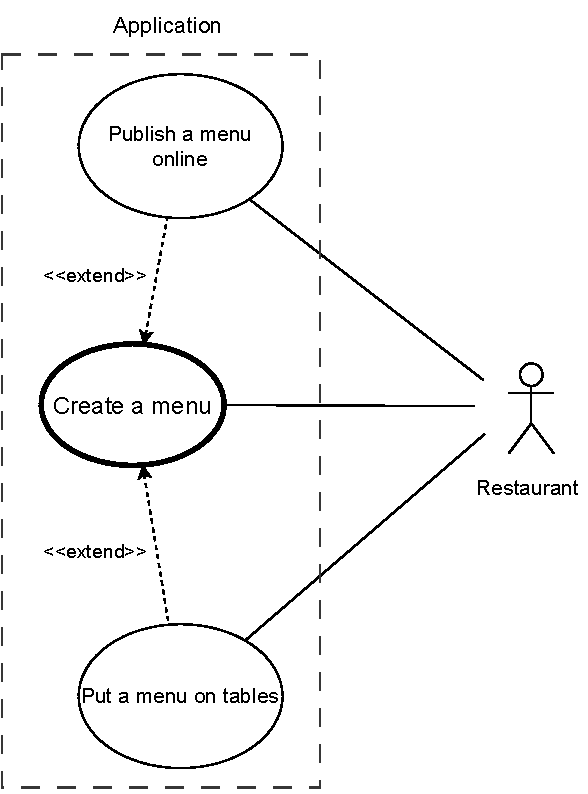
\includegraphics[width=0.62\linewidth]{master-thesis/img/use-cases/use_cases_restaurant_publish_menu}
  \caption{Restaurant offer use cases}
\end{figure}

\begin{figure}[h]
  \centering
  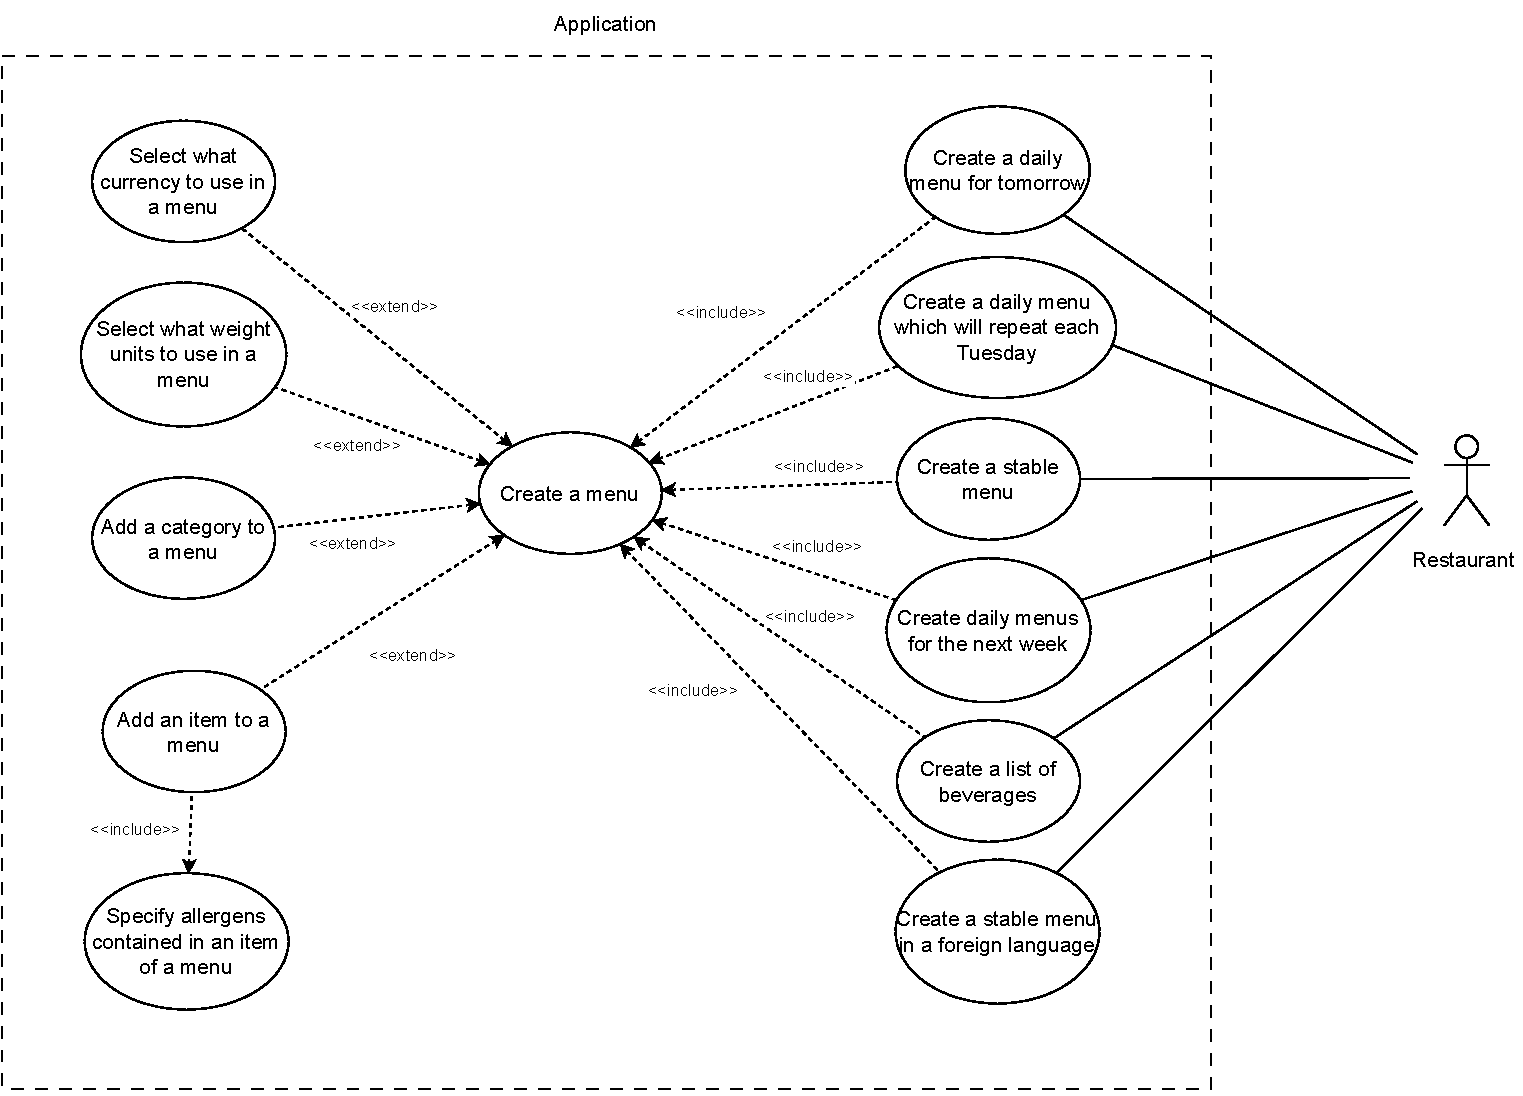
\includegraphics[width=0.62\linewidth]{master-thesis/img/use-cases/use_cases_restaurant_create_menu}
  \caption{Restaurant menu creation use cases}
\end{figure}

\begin{figure}[h]
  \centering
  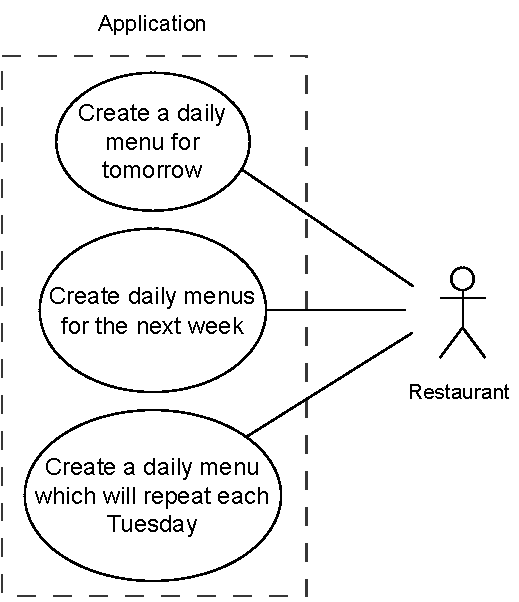
\includegraphics[width=0.62\linewidth]{master-thesis/img/use-cases/use_cases_restaurant_create_daily_menu}
  \caption{Restaurant daily menu creation use cases}
\end{figure}
